\documentclass{beamer}
\mode<presentation>
{
  \usetheme{default}      
  \usecolortheme{default} 
  \usefonttheme{default}  
  \setbeamertemplate{navigation symbols}{}
  \setbeamertemplate{caption}[numbered]
} 

\usepackage[english]{babel}
\usepackage[utf8x]{inputenc}
\usepackage{graphicx}
\usepackage[font=scriptsize,labelfont=scriptsize]{caption}
\usetheme{metropolis}

\title{fed2vec: a machine learning approach to forward guidance and market expectations}
\author{Temitope Akashoro\\
		Scott McNeil}
\date{\today}

\begin{document}

\begin{frame}
  \titlepage
\end{frame}


\begin{frame}{Motivation: FOMC and Forward Guidance}

\begin{columns}
	\begin{column}{0.5\textwidth}
		\begin{itemize}
			\item FOMC releases statements after meetings, detailing future policy
			\item Previous research (Campbell et al. 2012, Gurkaynak et al. 2005) study federal fund futures (FFF) as proxy
			\item Can we directly study these statements and their impact on market expectations?
		\end{itemize}
	\end{column}
	\begin{column}{0.5\textwidth}
		\begin{figure}
			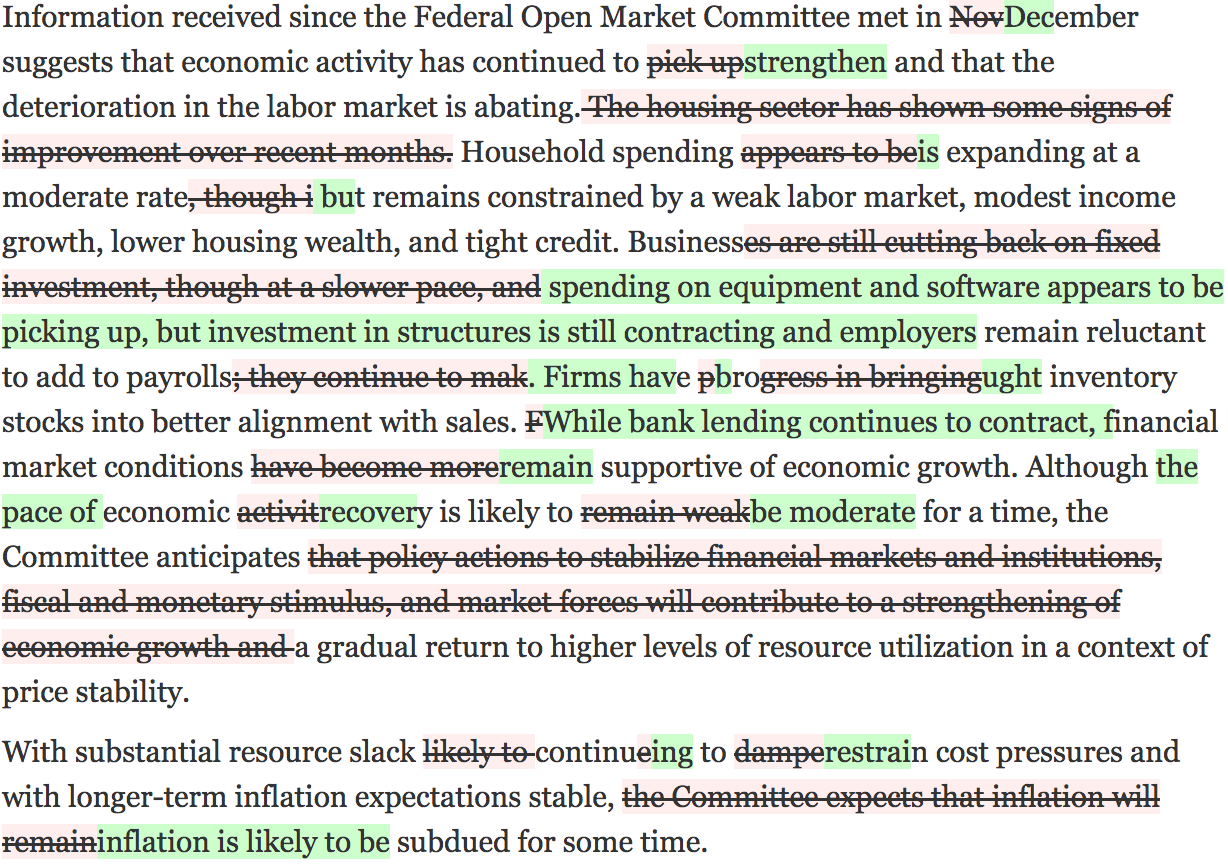
\includegraphics[width=1.05\textwidth]{fomcstatement.png}
			\caption{The \emph{Wall Street Journal's} \textquotedblleft Fed Statement Tracker\textquotedblright}
		\end{figure}
	\end{column}
\end{columns}

\end{frame}


\begin{frame}{word2vec and doc2vec}

\begin{columns}
	\begin{column}{0.5\textwidth}
		\begin{itemize}
			\item Mikolov, et. al. (2013) and Le and Mikolov (2014) present word and document \textquotedblleft vectorization\textquotedblright
			\item Learn representation via word co-occurrence
			\item Vectors (and distances between vectors) encode semantics
		\end{itemize}
	\end{column}
	\begin{column}{0.5\textwidth}
			\begin{figure}
				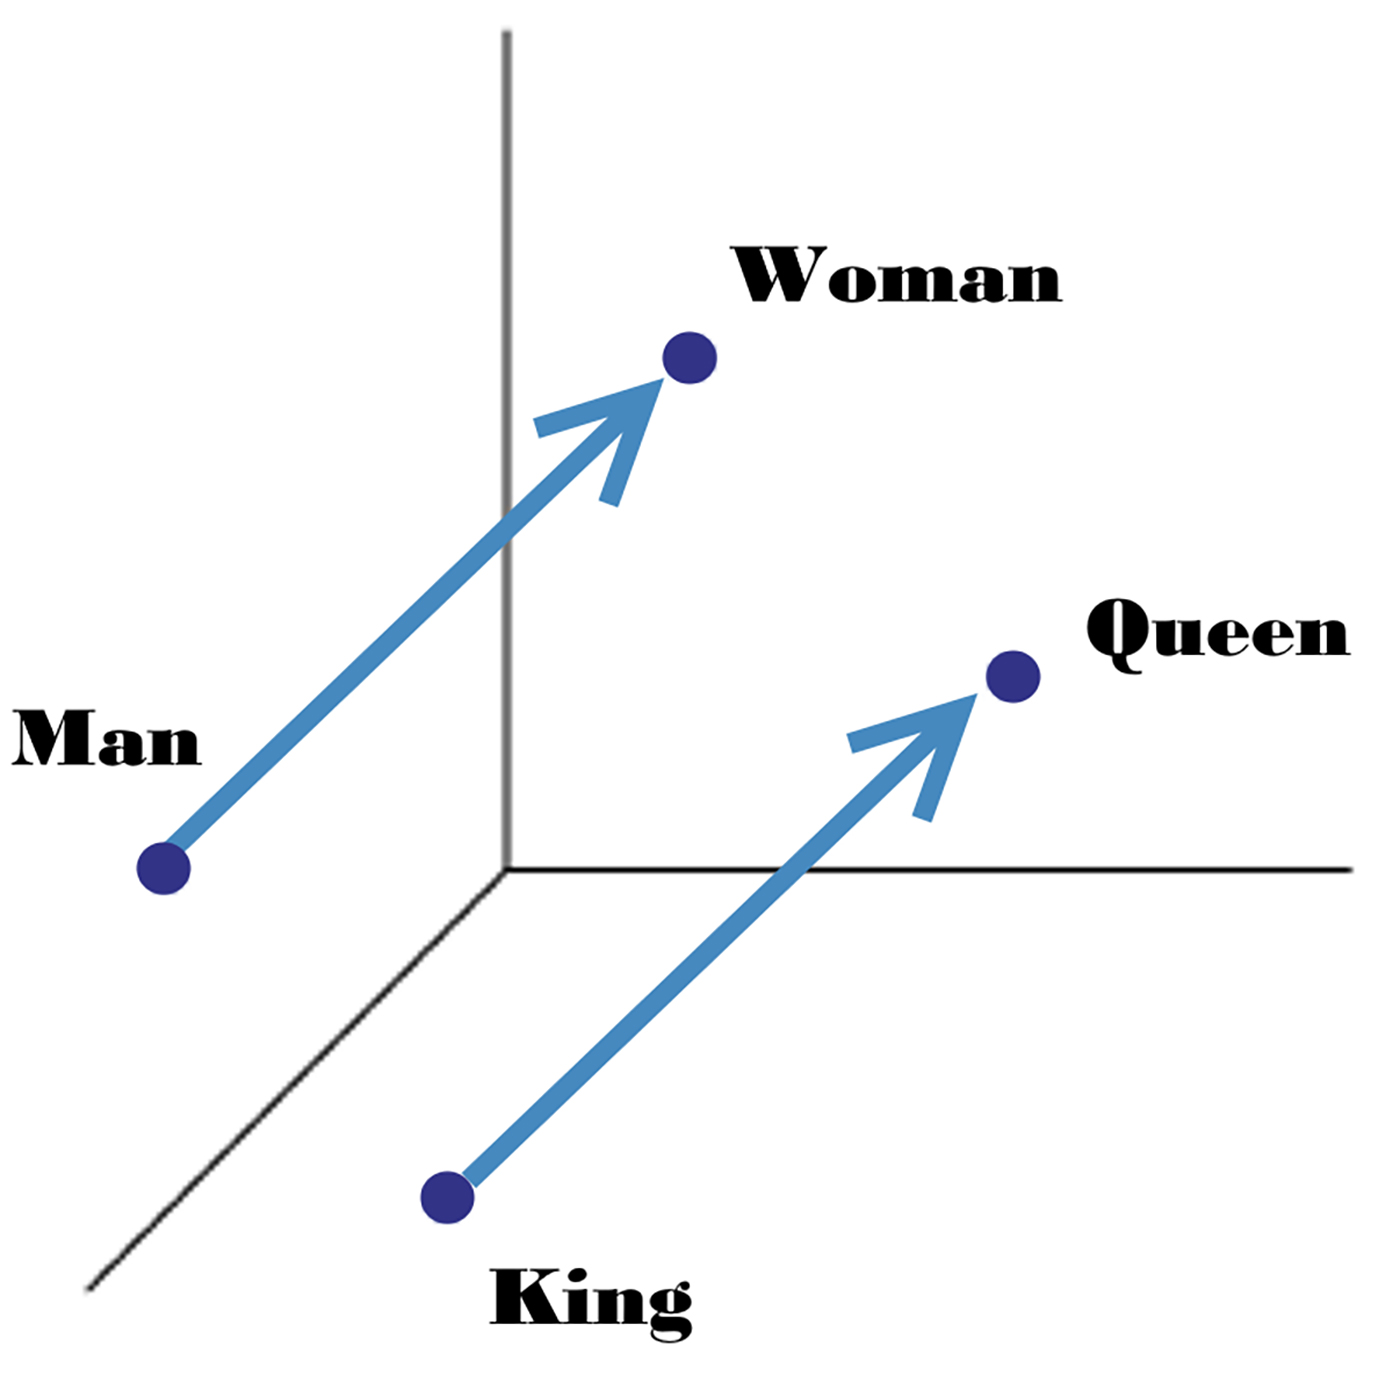
\includegraphics[width=\textwidth]{wordembedding.jpg}
				\caption{Result from Mikolov, et. al. (2013): king - him + her $\approx$ queen}
			\end{figure}
	\end{column}
\end{columns}


\end{frame}

\begin{frame}{Factor Augmented Vector Auto-regression (FAVAR)}
	
	\begin{columns}
		\begin{column}{0.48\textwidth}
			\begin{itemize}
				\item FFF, statements, real economy all endogenous\quad $\Rightarrow$ SVAR model
				\item FAVAR uses PCA to preserve degrees of freedom (e.g. Bernanke et al. 2004)
				\item Use for real economy and semantic data
			\end{itemize}
		\end{column}
		\begin{column}{0.5\textwidth}
			 \scriptsize\begin{align}
			&A\begin{bmatrix}
			\hat{S}_t\\\hat{F}_t\\\-\Delta FFF_t
			\end{bmatrix} =
			B\begin{bmatrix}
			\hat{S}_{t-1}\\\hat{F}_{t-1}\\\Delta FFF_{t-1}
			\end{bmatrix} + \epsilon_t \nonumber \\
			&\hat{S}_t\text{: $m\times1$ vec. of est. semantic factors} \nonumber \\
			&\hat{F}_t\text{: $k\times1$ vec. of est. real-economic factors} \nonumber \\
			&\Delta FFF_t\text{: change in federal funds futures rate} \nonumber \\
			&\epsilon_t\text{: vec. of innovations} \nonumber \\
			&A\text{: $m+k+1$ square matrix of contemp. coeff.} \nonumber \\
			&B\text{: $m+k+1$ square matrix of lag coeff.} \nonumber
			\end{align}
		\end{column}
	\end{columns}
\end{frame}


\begin{frame}{References}
\nocite{gurkaynak2005actions}
\nocite{campbell2012macroeconomic}
\nocite{le2014distributed}
\nocite{mikolov2013efficient}
\nocite{bernanke2005measuring}

\setbeamertemplate{bibliography item}[text]
\setbeamerfont{bibliography item}{size=\scriptsize}
\setbeamerfont{bibliography entry author}{size=\scriptsize}
\setbeamerfont{bibliography entry title}{size=\scriptsize}
\setbeamerfont{bibliography entry location}{size=\scriptsize}
\setbeamerfont{bibliography entry note}{size=\scriptsize}
\bibliographystyle{plain}
\bibliography{references}

\end{frame}
\end{document}
